\chapter{Programming documentation}
\label{chap:prog_docs}

This chapter will introduce the reader to the code changes made to the original PrankWeb interface. The first part will focus on the frontend, the second part will focus on the plug-ins.

\section{Frontend}
\label{sec:frontend}

The frontend of PrankWeb works as a TypeScript application. TypeScript is transpiled to JavaScript and bundled using Webpack. The application uses React for rendering a panel containing a tool box (see \cref{fig:toolbox}), structure information and pocket data. Styles are provided by CSS files and SCSS Bootstrap. All packages used in PrankWeb are installed using the npm tool. This architecture was already present in the original interface.

\begin{figure}[ht]
    \centering
    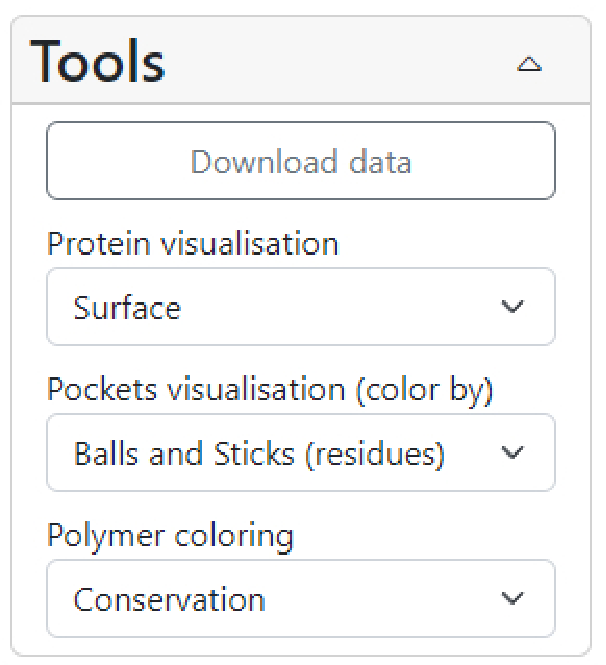
\includegraphics[width=0.4\linewidth]{img/toolsbox.pdf}
    \caption{The tool box component.}
    \label{fig:toolbox}
\end{figure}

The former interface was based on the LiteMol library for visualizing the structure. LiteMol is no longer developed, so one of the goals was to replace this plug-in with a new, modern structure viewer from the same authors - MolStar. Not only have the visuals significantly improved, the overall performance of MolStar is also much better. \cite{10.1093/nar/gkab314}

Before the current change, PrankWeb used a different library for rendering the 1D sequence visualization. The original implementation used the Protael library for a simple visual representation of the pockets, binding sites and scores. This library is intended for creating customizable visualizations for a protein structure \cite{10.1093/bioinformatics/btv605}. Protael is an old plug-in and in the original implementation, it needed to be modified in a significant way to fit the needs of PrankWeb. The new implementation presented in this thesis uses the RCSB Saguaro 1D Feature Viewer, which provides a more convenient way to display the pockets, binding sites and scores. \cite{10.1093/bioinformatics/btaa1012}

\subsection{High-level overview}
\label{subsec:frontend-overview}

Firstly, let's describe the typical data flow between the frontend and backend. Assuming that this section works with the \texttt{frontend} folder of the repository, this folder contains all of the frontend logic including plug-in configuration files for Webpack and static assets. The static assets are located in the \texttt{public} subfolder. Those include several libraries (such as jQuery), CSS files and static images.

Moving onto the visualization logic to the \texttt{viewer} subfolder, the user starts at the \texttt{index.js} page, where they enter either a protein structure file or a RCSB protein identifier. A request via REST API is then sent from the frontend to the backend workers. If there is a free worker, the job is immediately processed. If there are no free workers, the job is queued and processed as soon as a worker becomes available. The backend workers then process the job and create a result file (see \cref{subsec:executor-p2rank} for details). Right after the request, the user is redirected to the \texttt{analyze.ts} file. The frontend periodically fetches both the status file and the log file to display the current job progress. When the job is finished, the user is redirected to the \texttt{viewer.ts} file. The entrypoint to the viewer is the \texttt{renderProteinView} method, which will be covered later on. The viewer file is responsible for visualizing the structure, the pockets, binding sites and scores. The last step is to combine the plug-ins together, so that the user can interact with the structure and the data.

\subsection{MolStar}
\label{subsec:frontend-molstar}

MolStar (also Mol*) is a TypeScript library for visualizing protein structures. MolStar combines the strengths of the LiteMol and NGL libraries to provide a high-performance tool for bioinformatic scientists. The library is open-source and the code may be found on GitHub\footnote{https://github.com/molstar/molstar}. One downside of MolStar is that it lacks detailed documentation. There are some examples available in the GitHub repository either directly in the source codes or in issues, but for more complicated code, the user may need to create their own issue and ask the developers directly. An example of the visualization is shown in \cref{fig:molstar}.

\begin{figure}[htb]
    \centering
    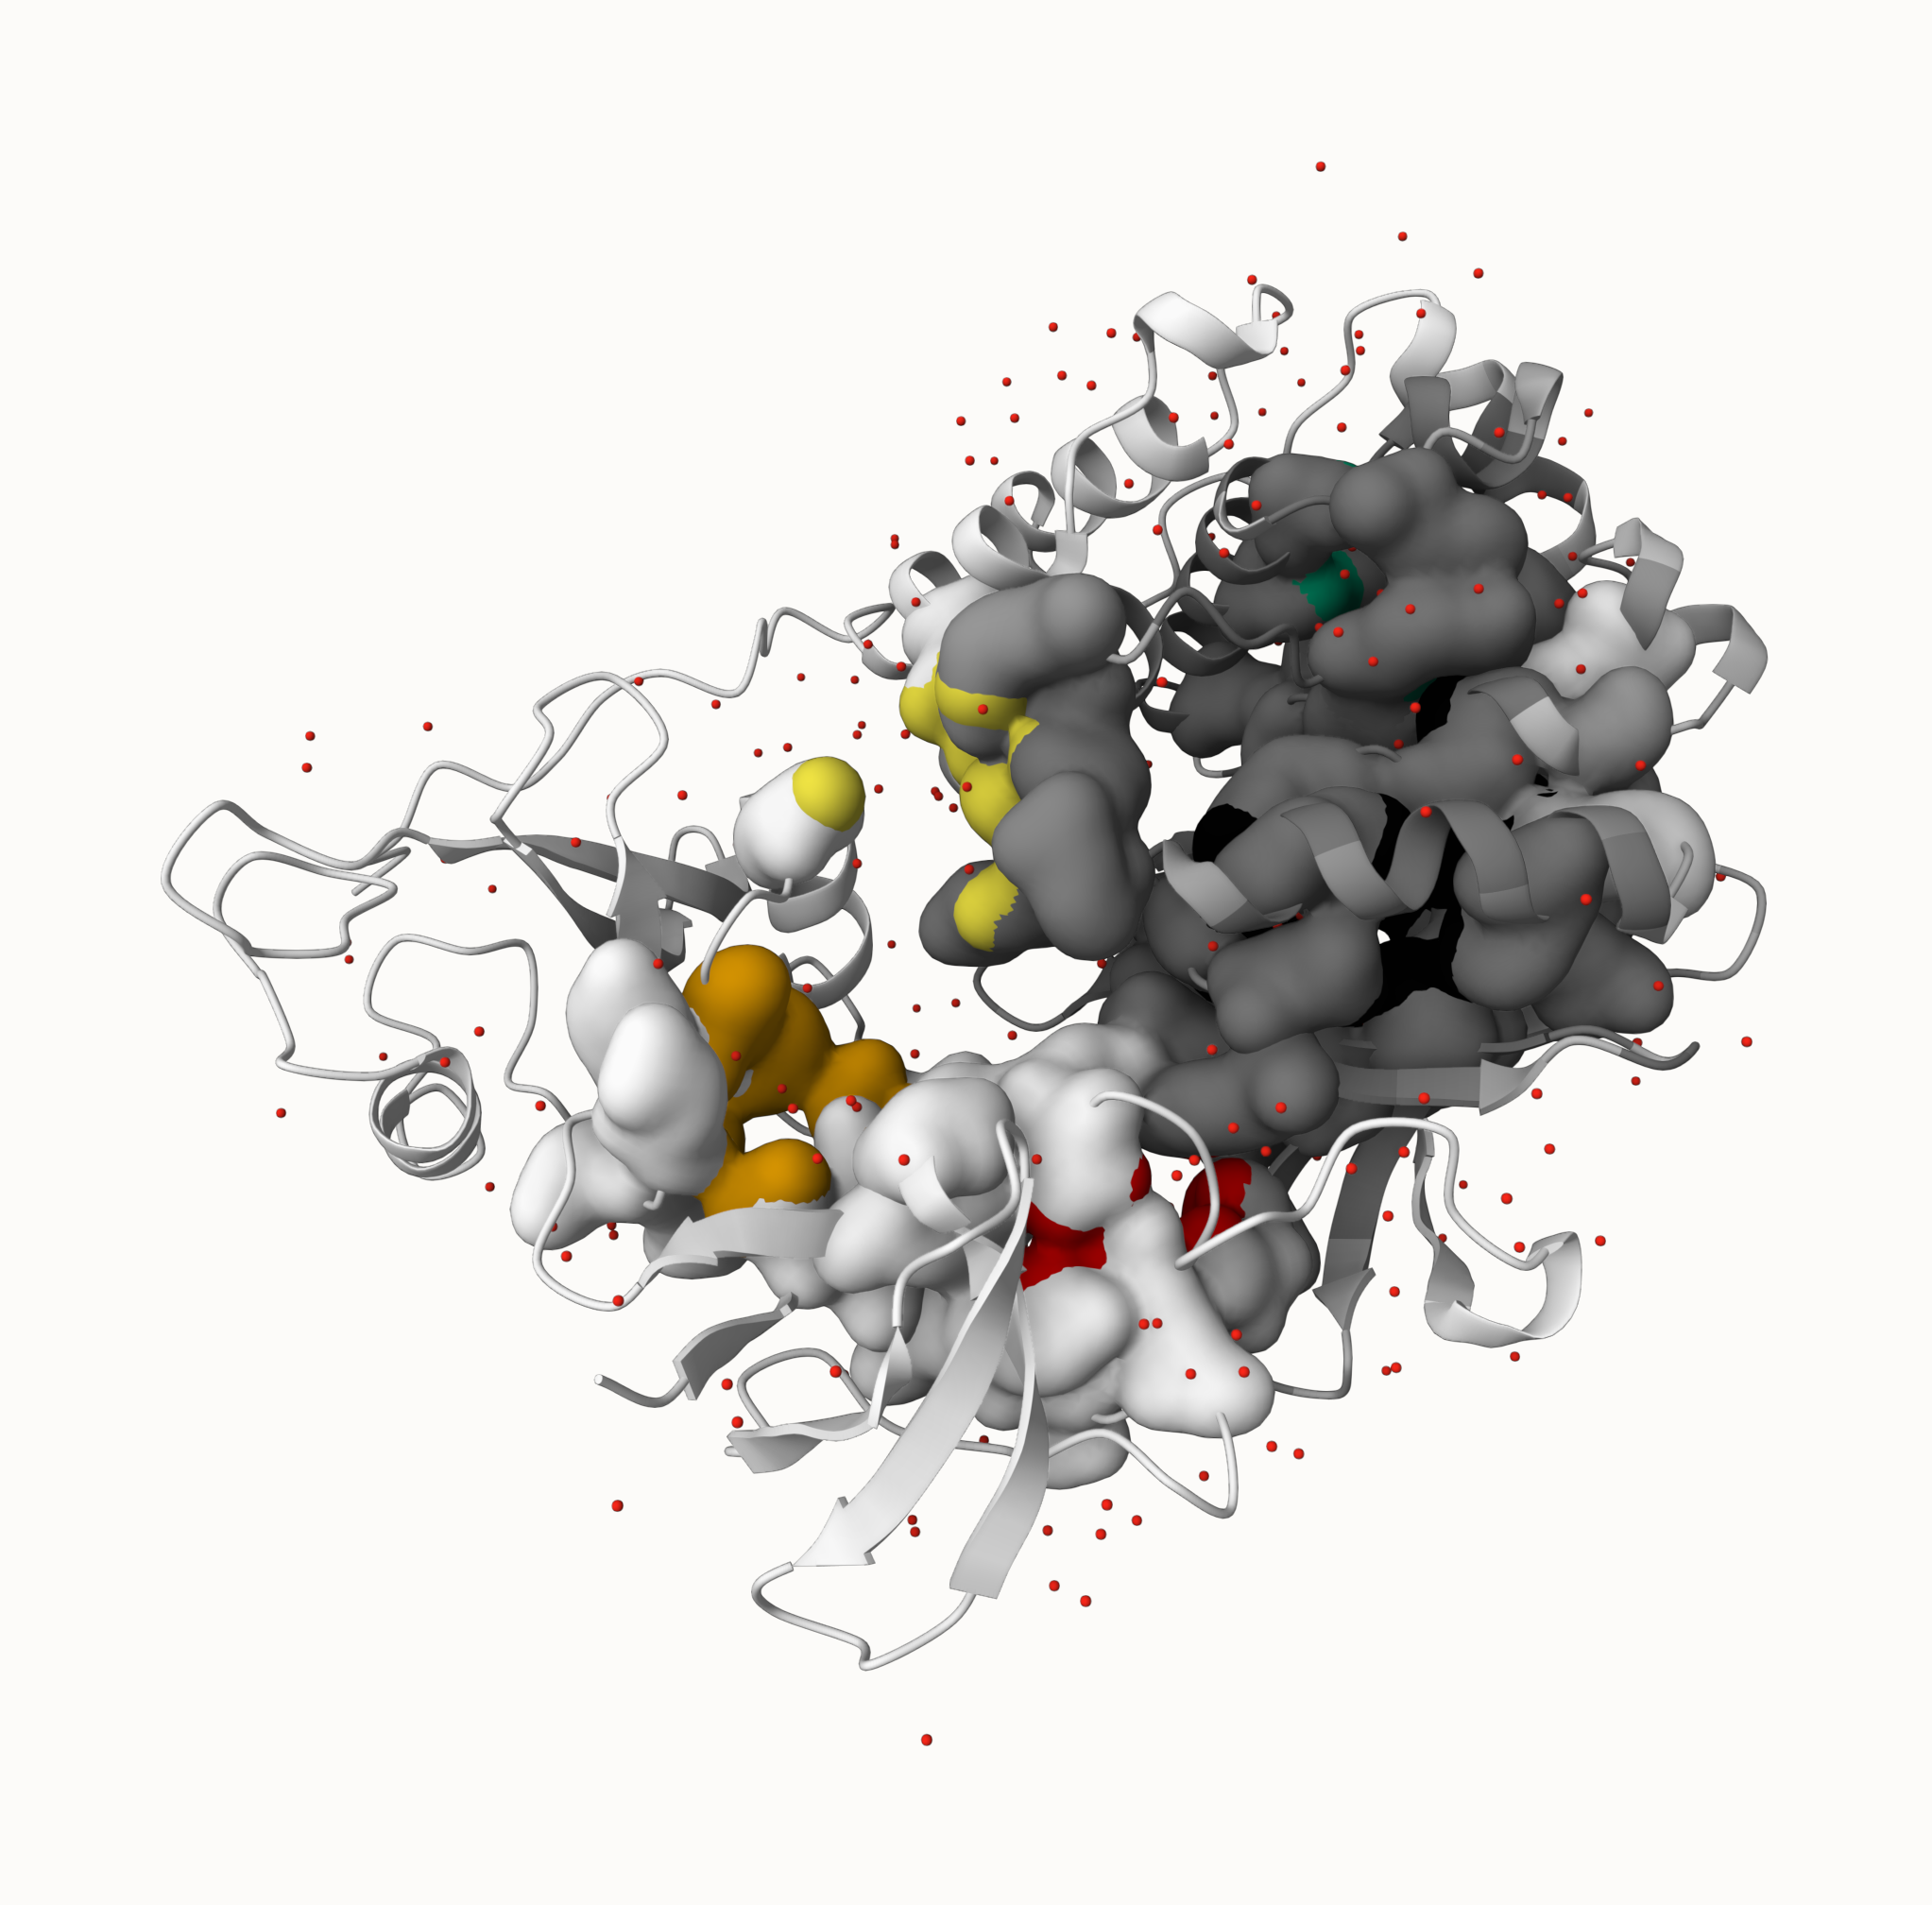
\includegraphics[width=\textwidth]{img/molstar_2src.png}
    \caption{A screenshot of the MolStar viewer for the \texttt{2SRC} structure. The structure is shown in cartoon representation and is colored by the conservation score. The pockets are shown in the surface representation.}
    \label{fig:molstar}
\end{figure}

After invoking the \texttt{renderProteinView} method, a MolStar viewer instance is created by calling the \texttt{createPluginUI} method from the library. An instance of \texttt{PluginUIContext} is returned. This instance is saved and used throughout the entire existence of the session. After the initialization, the main React component called \texttt{Application} is rendered for the first time. After mounting the component, the main visualization method \texttt{sendDataToPlugins} is called. This method from \texttt{data-loader.ts} is responsible for sending the prediction data for both plugins.

Some of the mentioned methods were already present in previous versions of PrankWeb. One of the goals of this thesis was to integrate MolStar into PrankWeb by replacing LiteMol. This lead to removal of the original LiteMol related code and introduced a few changes to the existing methods loading data into the viewer. All of MolStar related code was written from scratch to fit the needs of PrankWeb. Most of the code related to MolStar is located in the \texttt{molstar-visualise.ts} file. The following text describes the flow of the MolStar related interactions that create the core functionality of PrankWeb. These newly introduced methods call the MolStar library methods to create the visualization just from the data available in the prediction file and the structure file.

Firstly, the program asks for the API endpoint URL which resolves to a structure file. This file is loaded into MolStar via the \texttt{loadStructureIntoMolstar} method. This method parses the structure based on the file format and creates all of the available representations, such as surface, cartoon and ball-and-stick. It also tries to show the water molecules and ligands, if there are any.

When the structure is successfully shown to the user, a prediction is fetched from the API. Then, the 1D viewer is initialized. The 1D viewer connects to the MolStar plugin via callbacks. When the user hovers over a residue in the 1D viewer, the residue is highlighted in the MolStar plugin as well. When the user clicks a residue (or a pocket block), then the specific residue is focused in the MolStar plugin. The 1D viewer calls the \texttt{highlightInViewerAuthId} and \texttt{highlightInViewerLabelIdWithoutFocus} methods. See \cref{subsec:frontend-saguaro} for more details about the code that explains the interactions between the 1D viewer and the MolStar plugin.

After initializing the viewer and visualizing the structure, we need to show the pockets as well. The current implementation uses the following procedure: process every of the pockets and create a custom colored representation that will be added to the visualization. This is done in the \texttt{createPocketsGroupFromJson} method, which simply invokes \texttt{createPocketFromJson} for each of the pockets. That method creates multiple representations to allow the user to decide between various ways to display the pocket. Currently, a ball-and-stick and surface representations colored by either surface atoms or the entire residues are available. In future, more representations may be added. By default, only the surface atoms are shown as a pocket. The representations are added to a global variable containing all of them to allow switching between them based on user inputs from the React components.

For predicted structures, there is a special case. The predicted structure may contain areas that have not been properly analyzed, because no similar structures may be known. So, each of the resiudes is ranked with an AlphaFold pLDDT score that indicates how well a residue is predicted. Residues ranked with a score below 70 are ranked as low-confidence. \cite{jumper2021highly} PrankWeb enables the user to hide these residues from the visualization. This is done by creating a second structure visualization containing only the high-confidence residues. The user can switch between the two visualizations using a React component. For the creation of the second structure, we employ the \texttt{addPredictedPolymerRepresentation} method, which works in a similar way as creating the pockets.

After resolving the predicted structure, we have to ensure only the selected representations are visible to the user to ensure the best performance. This is done via the \texttt{showAllPocketsInRepresentation} method. Then, MolStar has to be linked to the 1D viewer, but in the opposite direction. Hovering over a residue in MolStar should highlight the corresponding residue in the 1D viewer. The method is called \texttt{linkMolstarToRcsb} and uses MolStar hover callbacks to achieve this behavior. The code is inspired by the MolArt library. \cite{molart}

In the last step, it is necessary to compute an average conservation (and potentially pLDDT) scores for each of the pockets. The JSON file provided by P2Rank contains the average scores only at the residue-level, so the pocket-level average needs to be computed. As we assume that the pockets are not large, this computation is done in the frontend and is not cached in any way. This is done in the \texttt{computePocketConservationAndAFAverage} method.

In this step, the MolStar visualization is complete and ready-to-use. The user may interact with the structure either via the 1D viewer, or via the MolStar plugin, or via the React components. The last part of the code is responsible for enabling interactions with the React tools. Currently, the user may interact with MolStar from the components in the following ways:

\begin{itemize}
    \item Change structure representation
    \item Change pockets representation
    \item Color residues by conservation or pLDDT scores
    \item Hide low-confidence residues for predicted structures
    \item Hide/show all pockets
    \item Hide/show individual pockets
    \item Highlight a pocket including zoom
\end{itemize}

All of the interactions are handled by calling the respective methods directly from the React components, which are described in \cref{subsec:frontend-react}. We will not cover details of the code, as it is mostly straightforward and the code is documented. The main idea is to apply transforms to the MolStar structure which is then re-rendered by the library.

In the end, we will show a brief code structure of the \texttt{molstar-visualise.ts} file containing the vast majority of MolStar-related code, just to give an overview of the MolStar integration.

\lstinputlisting[language=JavaScript,caption={
    A slightly edited version of a declaration file \texttt{molstar-visualise.d.ts}.
}]{code/molstar-visualise.d.ts}


\subsection{RCSB Saguaro 1D Feature Viewer}
\label{subsec:frontend-saguaro}

Alongside to the MolStar plugin, we use the RCSB Saguaro 1D Feature Viewer to display the pockets, actual binding sites and scores in a simple view mapped to the residues, which is the key feature of this plugin. The viewer is designed to easily identify multiple annotations on a single residue.

The RCSB Saguaro 1D Feature Viewer is a TypeScript library for visualizing protein features in a 1D view. An example usage is shown in \cref{fig:1d-viewer}. The code is available on GitHub\footnote{\url{https://github.com/rcsb/rcsb-saguaro}}. Documentation is available and the usage is simple, but it is important to keep in mind that the library is still under active development and the interface may change in the future.

\begin{figure}[htb]
    \centering
    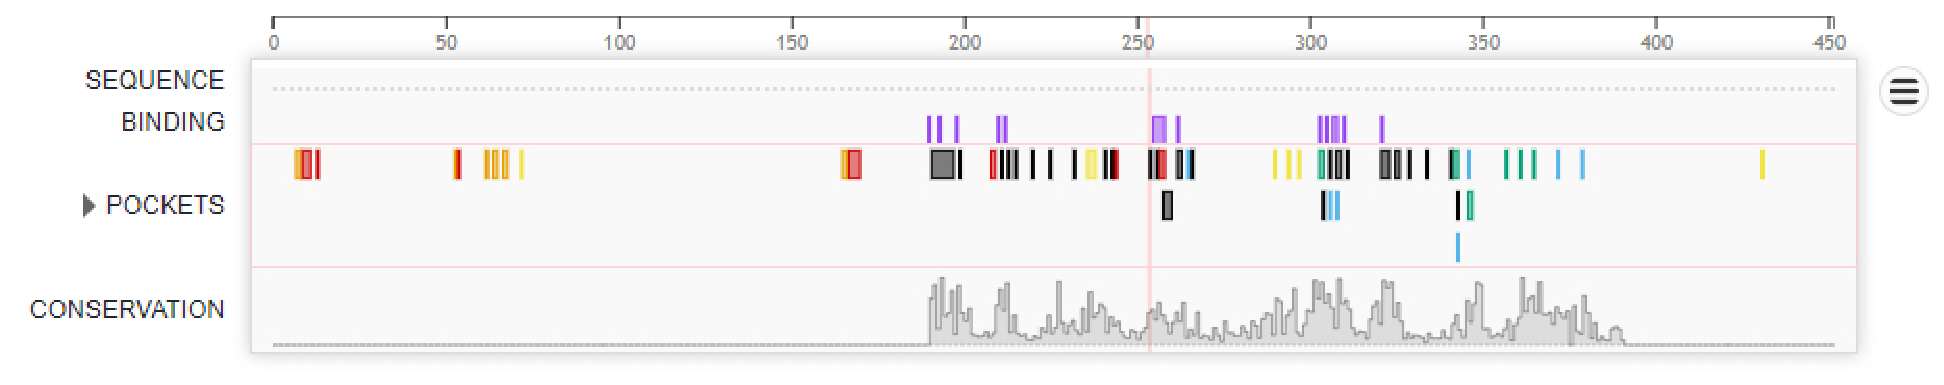
\includegraphics[width=\linewidth]{img/rcsb_2src.pdf}
    \caption{The RCSB Saguaro 1D Feature Viewer for the \texttt{2SRC} structure.}
    \label{fig:1d-viewer}
\end{figure}

In the original PrankWeb implementation, Protael was used for mapping the annotation to the single residues. In this thesis, we decided to use the RCSB Saguaro 1D Feature Viewer instead. The main reason for this decision is that the RCSB Saguaro 1D Feature Viewer is a more extensible library and is actively maintained. So, all of the code related to Protael was removed and replaced with new code using the RCSB Saguaro 1D Feature Viewer to provide the same functionality.

Most of the methods are defined in the \texttt{rcsb-visualise.ts} file. In our case, as described in \cref{subsec:frontend-molstar}, the 1D viewer gets initialized by the \texttt{sendDataToPlugins} method. This calls the \texttt{initRcsb} method which prepares all of the data for the plug-in.

The first thing to notice is calculating the viewer actual width. This is done in the \texttt{calculateViewerWidth} method. Unluckily, the viewer allows only a fixed width measured in pixels. This is a problem, as the viewer is not responsive and every time the user resizes the window, the viewer would have to be re-initialized, which would be pretty inefficient. So, for the first time the page loads, we calculate the width of the viewer based on a knowledge of the desired width that is set via CSS. We also have to subtract a certain amount of pixels to account not only for the viewer itself, but also for the margins, paddings and a custom viewer scrollbar, which is, once again, in-built in the viewer and is not customizable. We discussed this issue and came to a conclusion that the best solution is to add better-looking custom scrollbars to the viewer to provide a better user experience until the viewer is made responsive.

Then, the RCSB board is configured to interact with the MolStar viewer. This is done via the \texttt{onHighlight} and \texttt{elementClicked} methods. The first method is called when the user hovers over a certain residue in the 1D viewer. The actual callback is debounced to prevent lagging. A request for highlighting the specific residue in MolStar is then sent. The second method is called when the user clicks on a residues in the 1D viewer. A similar request is sent to MolStar with the difference that the residue is also zoomed in.

The last step is to prepare the actual data for each of the so-called tracks. A track represents one row (or multiple rows) containing information about a specific annotation. This is done in the \texttt{createRowConfigDataRcsb} method. A sequence track simply contains the protein amino acids. The binding track contains the actual binding sites computed by P2Rank. Pocket tracks are distinguished by different colors, which are picked firstly based on color-blind schemes to ensure the best accessibility, secondly randomly. The pocket color is changed in the original pocket data as well, so that the same colors for the pockets are used throughout the application. The last tracks are the conservation and pLDDT tracks, if available. Computation of the pocket tracks is not simple and straightforward, as the JSON file provided by P2Rank does not fit the viewer's interface, so the method highly relies on the JSON structure.

The 1D viewer does not rely on any React components and the only interaction may be done via the MolStar plugin simply by hovering over the residues, as described in \cref{subsec:frontend-molstar}.

Similarly to MolStar, let's have a look at the \texttt{rcsb-visualise.ts} file structure and the most important methods.

\lstinputlisting[language=JavaScript,caption={
    A slightly edited version of a declaration file \texttt{rcsb-visualise.d.ts}.
}]{code/rcsb-visualise.d.ts}


\subsection{React components}
\label{subsec:frontend-react}

This section will describe the React components that are related to the structure visualization. Most of the components were already present in the previous version of PrankWeb, but there was a need to refactor them to make them more modular and reusable, as well as to add new features and improve the user experience.

The application uses the following components:

\begin{itemize}
    \item \textbf{Application} - the main component of the app, responsible for the overall structure of the page including the viewers
    \item \textbf{ToolBox} - a component containing tools for changing the structure representation, coloring residues, hiding low-confidence residues and downloading data
    \item \textbf{StructureInformation} - a component containing the structure name
    \item \textbf{PocketList} - a component containing a list of all pockets with their scores and a button for hiding/showing all of them
    \item \textbf{Pocket} - a component containing a single pocket with its information and buttons for hiding/showing the pocket, highlighting the pocket and opening a dialog with the pocket details
    \item \textbf{PocketDetails} - a component defining the information of a Pocket component
    \item \textbf{PocketProperty} - a component visualizing a single property of a Pocket component
\end{itemize}

Other components will be covered in \cref{sec:plugins} as they are related to the plug-ins.

All React components are defined in their own files in the \texttt{components} subdirectory. The components extend the \texttt{React.Component} class to utilize the props and state features of React. The components invoke the responsible RCSB and MolStar methods on various value changes, clicks on buttons and other events. Some of the props get passed from the parent component to the children, which allows an easy communication between them and enforces best practices and minimizes code duplication. Some of the components have state variables as well that mostly indicate their current visibility. The components create a tree that is visualized in \cref{fig:react-molstar}.

The components are styled as Bootstrap cards and thus they are responsive. Although we expect the user to use PrankWeb mainly on a desktop computer, it is necessary to provide a good first experience when encountering the application on a smaller screen.

\xxx{TODO: maybe some more details?}

\xxx{TODO: add UML diagram}

\begin{figure}[htb]
    \centering
    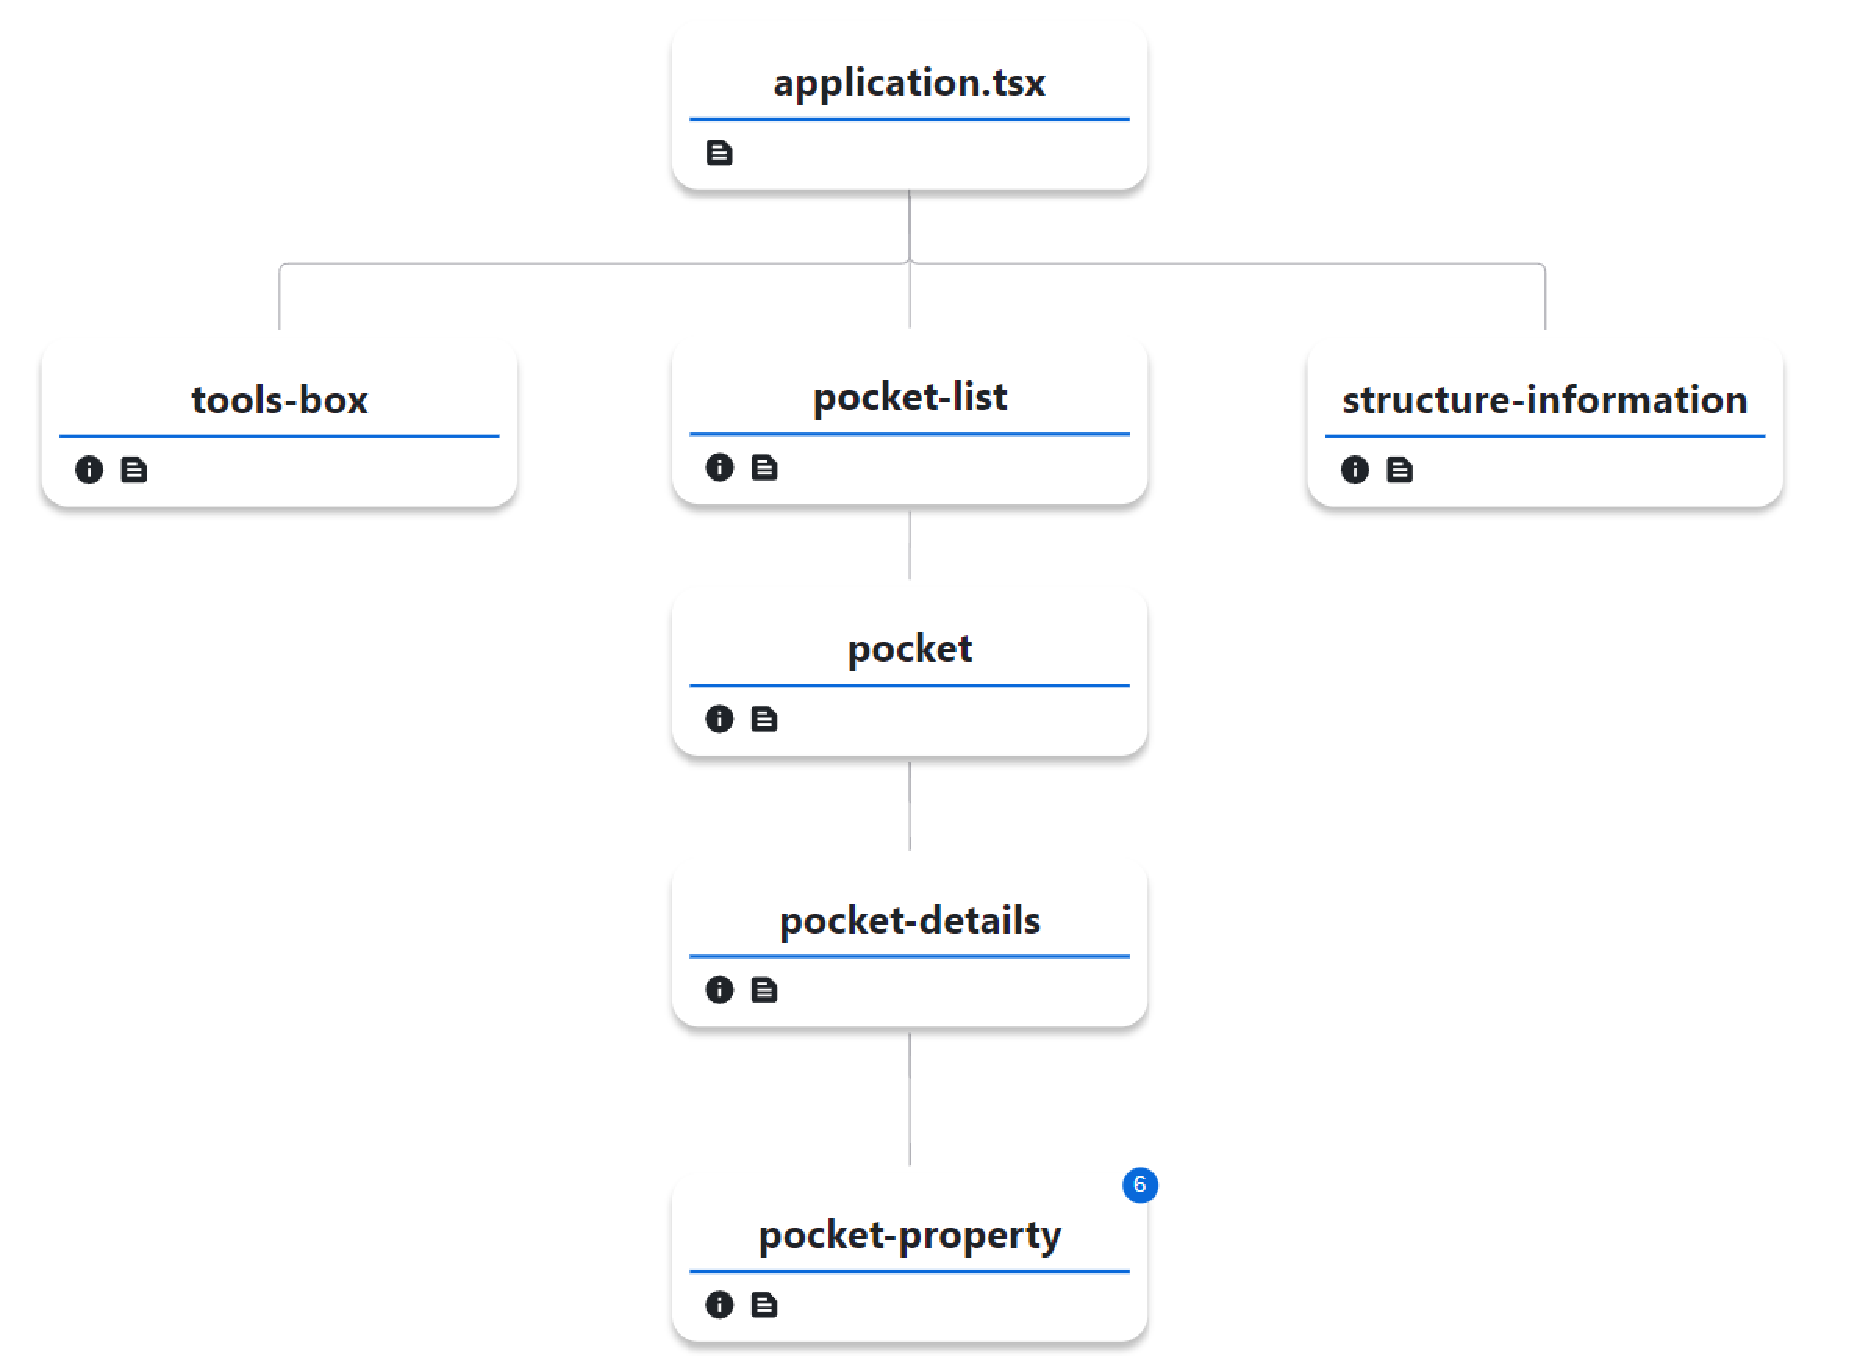
\includegraphics[width=\textwidth]{img/react_molstar.pdf}
    \caption{The React component tree showing only the components that are not related to the plug-ins.}
    \label{fig:react-molstar}
\end{figure}

\section{Plug-ins}
\label{sec:plugins}

The second goal of this thesis was to introduce a possibility to extend the current functionality of the application by adding new plug-ins (also called tasks). The plug-ins enable post-proccesing of the pockets. 

After a discussion, we created the following plug-in categories: client-side and server-side. It is assumed that the client-side plug-ins will be used for simpler tasks that may be computed from the existing data in each session, on the contrary the server-side plug-ins will be used for complex tasks that are more time-consuming and possibly utilize third-party software.

The PrankWeb interface for both of the tasks works as a set of React components that are modular, so new plug-ins may be introduced in an easy way without modifying much of the current code.

For an easy access to plug-ins, we have created a possibility to view the pocket details not only directly in the pocket list, but in a draggable dialog as well. This dialog is defined in the \texttt{DraggableDialog} and \texttt{PocketDialogDetails} classes that provide the implementation. The user may open multiple dialogs at once as well as drag them around the screen. The dialogs allow interaction behind them, so the user may still manipulate with both of the viewers.

This decision was discussed more and multiple designs were proposed and tested. All of the possible variants are listed in \cref{sec:pocket_detail_designs}. The final decision was made based on the fact that a vast majority of users is expected to use a big-screen device, so to keep the original usage easy and intuitive, we decided to keep the original design. One downside of this implementation is that the dialogs are not intended to be used on mobile devices. In other words, the dialogs are not available for small screens which makes this section irrelevant for those devices. On the other side, we believe that this is a reasonable trade-off.

In the following subsections, we will introduce the general plug-in interface and the implemented plug-ins.

\subsection{Client-side plug-ins}
\label{subsec:client-side-plugins}

The main intention of client-side plug-ins is to create a possibility to enable simple post-processing from the prediction data directly in the application. The tasks computed on client-side stay in the current session. 

Currently, the client-side plug-ins are defined in a \texttt{PocketDialogDetails} component as they are dialog-specific. A new interface for these plug-ins was created in the \texttt{PocketClientTask} component. Let's have a look at the interface.

\lstinputlisting[language=JavaScript,caption={
    An edited version of the \texttt{pocket-client-task.tsx} component.
}]{code/pocket-client-task.tsx}

Some of the props and state variables are self-explanatory, some of them are passed from the parent component. We will focus on the client-side specific props and state variables that define their behavior.

Firstly, let's take a look at the \texttt{taskType} prop. This prop defines the type of the task that is defined in the \texttt{ClientTaskType} enum. This enables a possible behavior difference of the client-side plug-ins based on their type. Next prop is a method called \texttt{compute}. This is the key method of the plug-in that provides the actual post-processing of the prediction data. The behavior is defined by the parent component. In the plug-in definition, the \texttt{compute} method is called. We expect this method to return a promise containing data conforming to the \texttt{ClientTaskData} interface. After receiving the result, the result needs to be rendered. During this entire process, state variables \texttt{taskData}, \texttt{computed} and \texttt{loading} are used to indicate the current computation progress.

Originally, one implementation for showing the result was created, but to provide a more generic approach to the problem, a second method was introduced to the props - the \texttt{renderOnComplete} method. This method takes the computed data as a parameter and returns a JSX component that renders the data inside the original dialog.

Currently, the client-side plug-ins are defined in the \texttt{tasks} subdirectory. The actual implementations are \texttt{.tsx} files and should contain both of the methods for the computation and rendering to keep the code clean.

As an example of a client-side plug-in, we have implemented a plug-in that computes the expected volume of the pocket. For this purpose, we have created a \texttt{tasks/client-atoms-volume.tsx} file that contains \texttt{computePocketVolume} and \texttt{renderOnTaskVolumeCompleted} methods that conform to the \texttt{compute} and \texttt{renderOnComplete} props of the \texttt{PocketClientTask} component. In this post-processing, we are using a convex hull algorithm to get coordinates of the hull vertices. Then, we use a simple formula to compute the volume of the convex hull using the coordinates of the vertices based on triangulation of the hull \cite{zhang2001efficient}. The result is then rendered in the dialog as a simple number. This implementation saves the computed results in a hashmap directly in the implementation file. This is not the most efficient way to store the results, on the other hand, it is a simple solution that is sufficient for this use case.

Creating a custom new client-side plug-in is covered in detail in \cref{sec:developer}.

\subsection{Server-side plug-ins}
\label{subsec:server-side-plugins}

Server-side plug-ins create an opportunity to perform more complex post-processing that takes more time to compute. Our intention was to allow users to use third-party software for the post-processing. Server-side tasks are meant to be parametrized by the user in some way.

The plug-ins are define in a similar way as the P2Rank executor, which may be processed by Docker containers (as mentioned in \cref{sec:prankweb_arch}).

There are a few steps that have to be done to implement a new server-side plug-in. First, API endpoints for the plug-in as well as the folder and file structure need to be defined. This is done in the \texttt{web-server} folder in Flask. Usually, it is expected that Flask will prepare the needed directories and files for the actual Docker container. For this process, it is typical to create a new Python class to contain all of this logic.

Then, in the Celery client configuration file in Flask, new bindings are created for the new plug-in. This includes creating a new Celery queue as well as introducing a new task that gets executed on the backend identified by its name.

After completing all of the Flask tasks, a new Docker container has to be created. The container should install Python with Celery and any other tools needed for the post-processing. It is expected that a new \texttt{Dockerfile} will be created for this purpose. After setting up the container, Celery bindings have to be created in a similar way as in Flask. Then, any method may be called from this Celery binding. This means that the actual post-processing may be finally done here. The first option is to do this in Python entirely, but it is also possible to call any other tool from the container. The only requirement is to have everything set up properly. 

The Docker container is also responsible for saving the results of the post-processing. This means that either some of the Python files or the third-party tool itself has to save the results in the correct location. Keep in mind that the location is very likely to depend on the API endpoints defined in Flask. Now, the Docker container is ready to be used.

It is highly recommended to include the newly created container into the Docker-compose file. This makes the deployment easy and allows simpler testing of the new plug-in\footnote{With Docker-compose, it is possible to restart just one of the containers, which makes the debugging faster.}.

After completing all of the steps, the new plug-in should be ready to be used. The only thing left is to include the plug-in to the frontend. For the frontend interaction, a new React component was introduced.

\texttt{PocketServerParametrizedTask} is meant to be used for the server-side plug-ins that require some parameters to be set by the user. This component is used in \texttt{PocketDialogDetails} similarly to client plug-ins (more about dialog in \cref{subsec:client-side-plugins}). Let's have a look at the server plug-in component.

\lstinputlisting[language=JavaScript,caption={
    An edited version of the \texttt{pocket-server-parametrized-task.tsx} component.
}]{code/pocket-server-parametrized-task.tsx}

The component works similarly to the client-side plug-in component. There are two methods that are responsible for the computation and rendering of the results. One of the differences is that these two methods are now identifiable by a hash that has to be computed from the parameters before the actual computation. This hash is not only used for frontend identification, but also for the backend. This technique allows us to differ between multiple tasks of the same type with different parameters.

There are more state variables as well. \texttt{modalOpen} and \texttt{formData} were introduced for receiving an input from the user, the current implementation opens a modal dialog with a text area. The \texttt{hash} is then computed from the input stored in the \texttt{formData} variable.

As the task results are persistent on the server, a new variable called \texttt{serverTasks} was introduced in the main component of the app. This component then periodically checks for all computed tasks for the given structure. The objects in this array are mutable and are modified for the purpose of the frontend rendering, so only the response data for tasks completed in this session are saved.

This allows us to render the hashes of the tasks that were computed both in this session and in previous ones. For this purpose, a new component called \texttt{TaskList} was introduced to display the list of tasks. \xxx{TODO: maybe we won't use this component in the end, so mention that its just available but not used}

One last change was made to the \texttt{PocketDialogDetails} component. A new component \texttt{PocketRunningTasks} was created to display a list of tasks that are either running or completed in this session. This is done to make sure that the task results are available to the user in case the dialog is closed and reopened. Moreover, this allows the user to enter multiple parameters for the same task and see the results for all of them.

\xxx{TODO: add an example of a server-side plug-in - docking, as soon as its completed}

\xxx{TODO: consider whether it is a good idea to describe the docker side even more and include some examples?}